\documentclass[11pt]{beamer}
\usetheme{Darmstadt}
\usepackage[utf8]{inputenc}
\usepackage{amsmath}
\usepackage{amsfonts}
\usepackage{amssymb}
\usepackage{graphicx}
\usepackage[fontset=windows]{ctex}


\author{Eurake}
\title{Beamer In TexMaker}
\setbeamercovered{transparent} 
% 更改底部的导航条样式
%\setbeamertemplate{navigation symbols}{\ensuremath{\sum}} 
% 设置Beamer的logo
\logo{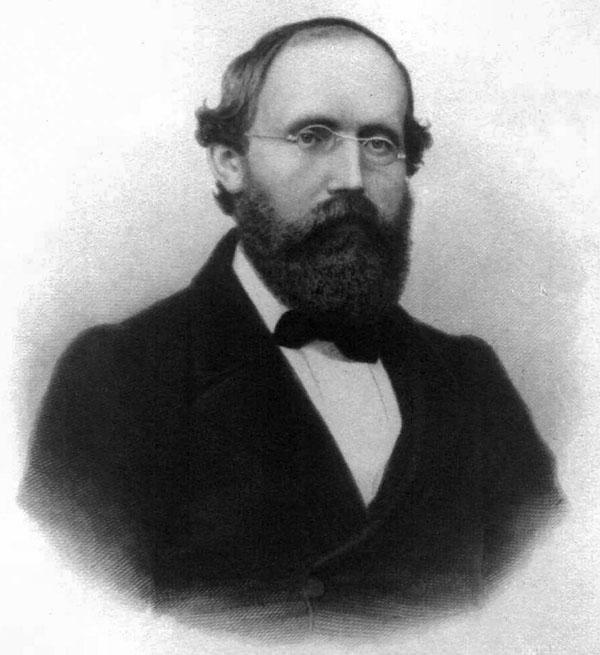
\includegraphics[scale=0.05]{./Dilichlet.jpg}} 
\institute{@ZHIHU} 
\date{\today} 
\subject{A Test About Texmaker} 


\begin{document}

	\begin{frame}
		\titlepage
		% 隐藏页眉,页脚
		\thispagestyle{plain}
	\end{frame}
	
	\begin{frame}
		\tableofcontents
	\end{frame}
	

	\begin{frame}
		\section{Test Theorem Env}		
		\begin{theorem}[Euler Equation]
			This is A Theorem Env, WHich Has Been Modified By \LaTeX Default
			\begin{align}
				\sum_{i=1}^{+\infty}{\frac{1}{i^2}}= \frac{\pi^2}{6}
			\end{align}
		\end{theorem}
		
		From The Env as before, we can conclude That: 
		The Theorem Env Won't go into Fomular By default.
	\end{frame}

	\section{制表使用}
	\begin{frame}
		\begin{tabbing}
		\hspace{16em}\=\kill
		 •The Fist \> • The Second\\
		 \bigskip\\
		 The First Info That Showning \> The Second Info  Showning\\
		 Above is Important \> Above is Important\\
		\end{tabbing} 
	\end{frame}

	\section{表格的使用}
	\begin{frame}
		\begin{tabular}{lr}
		\hline
		Element 1 & Elment 2\\ 
		\hline
		The $(1, 1)$ Element & The $(1, 2)$ Element \\ 
		\vspace{1em}\\
		The $(2, 1)$ Element & The $(2, 2)$ Element \\ 
		\hline 
		\end{tabular} 
	\end{frame}

\end{document}